\chapter{Μοντέλα μεταβλητότητας}

Προκειμένου να βγάλουμε συμπεράσματα για την σχέση της μεταβλητότητας συλλογών τουλάχιστον 20 πηγών (\textlatin{ensemble NXSV}) με θεμελιώδεις φυσικές παραμέτρους, όπως η μάζα κεντρικής μελανής οπής και ο ρυθμός προσάυξησης, θα συγκρίνουμε με μοντέλα μεταβλητότητας συλλογής \textlatin{AGN} που παρουσιάζονται στην εργασία <<\textlatin{Exploring black-hole scaling relations via the ensemble variability of Active Galactic Nuclei}>> (\textlatin{Georgakakis et al. 2021})\cite{VAR}. Τα μοντέλα αυτά κατασκευάστηκαν με βάση παρατηρησιακές σχέσεις.

%%------------------------%%
%%------------------------%%
%%------------------------%%
\section{Δόμηση μοντέλων μεταβλητότητας}

\begin{figure*}
 \begin{center}
 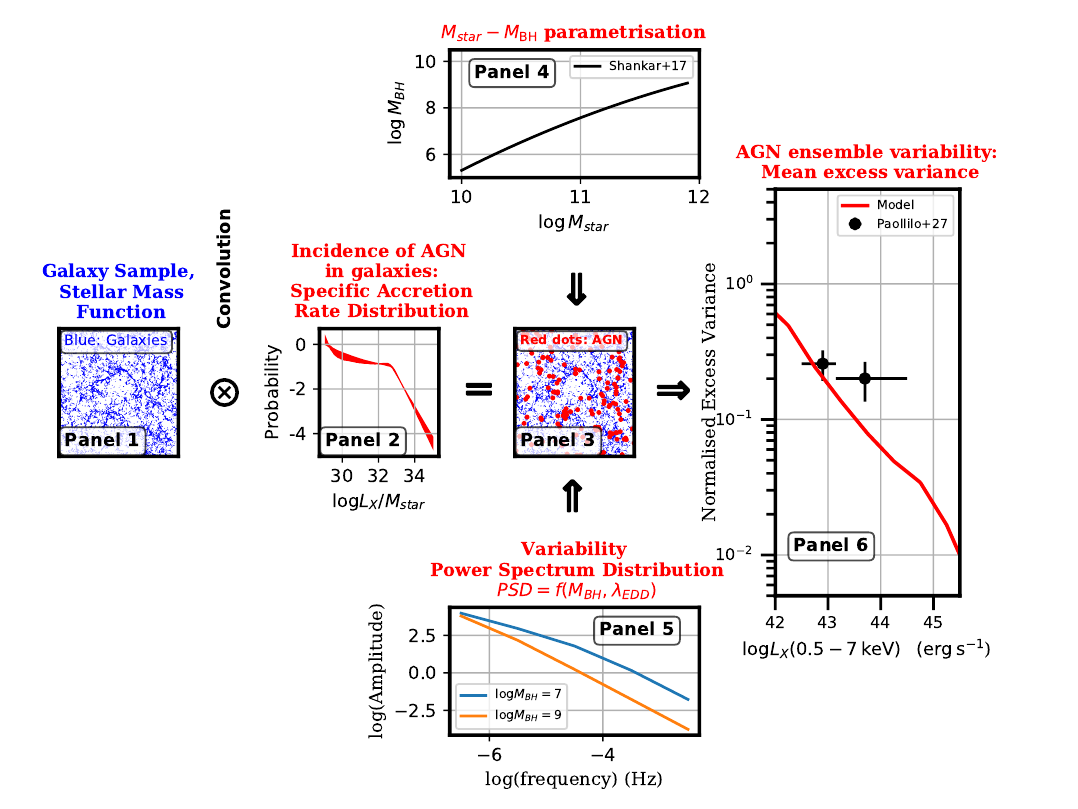
\includegraphics[width=1.1\linewidth]{Figures/ModelConstruction.png}
 \caption{\textlatin{Panel 1}: ογκική πυκνότητα γαλαξιών σε τμήμα κοσμικού ιστού. \textlatin{Panel 2}: πιθανότητα ένας γαλαξίας να έχει συγκεκριμένο ρυθμό προσύξησης. \textlatin{Panel 3}: κατανομή \textlatin{AGN} στην ογκική πυκνότητα γαλαξιών με αντίστοιχες τιμές παραμέτρων ($L_X$, $M_{\star}$, $z$).
 \textlatin{Panel 4}: προσθήκη πληροφορίας $M_{BH}$ και  $\lambda_{Edd}$ για το δείγμα, από την παραμετροποίηση μάζας κεντρικής μελανής οπής με αστρική μάζα γαλαξία και από την σχέση $\lambda_{Edd} \propto L_X/M_{BH}$. 
 \textlatin{Panel 5}: Μορφή συνάρτησης \textlatin{PSD} $\mathcal{P}(f)$ με εξάρτηση από τις φυσικές παραμέτρους του δείγματος (μάζας κεντρικής μελανής οπής $M_{BH}$ και ρυθμό προσύξησης $\lambda_{Edd}$).  
 \textlatin{Panel 6}: Ολοκλήρωση της \textlatin{PSD} στις χρονικές κλίμακες που μελετάμε για ευθύ υπολογισμό πλάτους μεταβλητότητας και σύγκριση με δεδομένα. (Εικόνα από \cite{VAR})}
 \label{fig:ModelConstruction}
 \end{center}
 \end{figure*}

%%------------------------%%

\subsection{Τεχνητός πληθυσμός \textlatin{AGN}}
Η κατασκευή τεχνητού πληθυσμού \textlatin{AGN} ξεκινά από ένα δείγμα γαλαξιών που ακολουθούν συγκεκριμένη συνάρτηση μάζας (όπως αυτό φαίνεται στο \textlatin{Panel 1} του σχήματος \ref{fig:ModelConstruction}) στους οποίους εφαρμόζεται η παρατηρησιακά καθοριζόμενη κατανομή ρυθμών προσαύξησης $\mathbf{p}(\lambda)$ για συγκεκριμένο ρυθμό προσαύξησης $\lambda \propto L_X/ M_{\star}$\cite{VAR}.
Όπου $\lambda$ ο ρυθμός προσαύξησης, $L_X$ η λαμπρότητα στις ακτίνες Χ σε δεδομένο φασματικό παράθυρο και $ M_{\star}$ η αστρική μάζα ενος γαλαξία. Η κατανομή $\mathbf{p}(\lambda)$ μετρά την πιθανότητα ένας γαλαξίας να φιλοξενεί έναν \textlatin{AGN} με ρυθμό προσαύξησης $\lambda \propto L_X/ M_{\star}$ (όπως αυτό φαίνεται στο \textlatin{Panel 2} του σχήματος \ref{fig:ModelConstruction})\cite{VAR}. Ο συγκεκριμένος ρυθμός προσαύξησης αυτός ($\lambda \propto L_X/ M_{\star}$) είναι μια παράμετρος που προκύπτει από παρατηρησιακά δεδομένα και είναι ένα μέτρο του πόση λαμπρότητα στις ακτίνες Χ παράγει ένας \textlatin{AGN} σε σχέση με την αστρική μάζα του γαλαξία που τον <<φιλοξενεί>>. Χρησιμοποιώντας αυτόν τον ρυθμό προσαύξησης στην $\mathbf{p}(\lambda)$, η κατανομή αυτή μας δίνει ένα μέτρο πιθανότητας να υπάρχει ενεργός γαλαξίας ανάμεσα σε πολλούς γαλαξίες. 
%({\color{red} με τη συναρτηση μαζας των γαλαξιων οχι την πυκνοτητα κοσμικου ιστου})
Έτσι η συνέλιξη της κατανομής πιθανότητας να υπάρχει \textlatin{AGN} με την γαλαξιακή πυκνότητα συγκεκριμένης συνάρτησης μάζας, μας δίνει μια χωρική κατανομή \textlatin{AGN} (όπως αυτή φαίνεται στο \textlatin{Panel 3} του σχήματος \ref{fig:ModelConstruction} με υπόβαθρο την γαλαξιακή πυκνότητα)\cite{VAR}. Το αποτέλεσμα είναι να έχουμε παράξει ένα τεχνητό δείγμα \textlatin{AGN} το οποίο είναι συνεπές με την εξελισσόμενη συνάρτηση λαμπρότητας ακτίνων Χ των \textlatin{AGN}, αναπαράγει την παρατηρούμενη συνάρτηση αστρικής μάζας των γαλαξιών με ενεργό γαλαξιακό πυρήνα, την χωρική κατανομή \textlatin{AGN} στον κοσμικό ιστό και τις ιδιότητες των \textlatin{AGN} σε όλα τα μήκη κύματος\cite{VAR}.
Κάθε σημείο στο τεχνητό αυτό δείγμα \textlatin{AGN} έχει αντίστοιχες τιμές λαμπρότητας $L_X$ (για την ενεργειακή μπάντα $2-10$ \textlatin{keV}), αστρικής μάζας γαλαξία $M_{\star}$ και \textlatin{redshift} $z$.

Ακολουθώντας την παραμετροποίηση μάζας κεντρικής μελανής οπής με αστρική μάζα γαλαξία, όπως αυτή φαίνεται στο \textlatin{Panel 4} του σχήματος \ref{fig:ModelConstruction}, αντιστοιχίζουμε σε κάθε \textlatin{AGN} με αστρική μάζα $M_{\star}$ μια τιμή μάζας κεντρικής υπερμεγέθους μελανής οπής $M_{BH}$. Στο τοπικό σύμπαν η αστρική μάζα του κεντρικού σφαιροειδούς των γαλαξιών συσχετίζεται στενά με την μάζα της κεντρικής μελανής οπής \cite{shankar}\cite{savorgnan}, στον αλγόριθμο παραγωγής τεχνητού πληθυσμού και μοντέλων για την \textlatin{ensemble NXSV} χρησιμοποιείται η συσχέτιση\cite{savorgnan}: 
$$\log_{10}\; \frac{M_{BH}}{M_\odot} = 8.35 + 1.31 \cdot \log_{10}\; \big( \frac{M_\star}{M_\odot} -11.0 \big)  $$
για να αντιστοιχίσουμε αστρικές μάζες του κεντρικού σφαιροείδούς με μάζες κεντρικών μελανών οπών. \\
%({\color{red} Αξιζει να πεις οτι στο τοπικο συμπαν η αστρικη μαζα του σφαιροειδους των γαλαξιων συνχετιζετασι στενα με τη μαζα της μαυρηα τρυπας και οτι αυτη τη συσχετηση χρησμοποιεις για να αντιστοιχισεις αστρικες μαζεσ μς μελανς οπες}).
Κατ> επέκταση, για κάθε τιμή φωτεινότητας $L_X$ που διαθέτουμε, αντιστοιχίζουμε μια τιμή πηλίκου \textlatin{Eddington} $\lambda_{Edd}$ σε κάθε ενεργό γαλαξιακό πυρήνα, me $\lambda_{Edd} \propto L_X/L_{Edd} \iff \lambda_{Edd} \propto L_X/M_{BH}$ , όπου $L_{Edd}$ η βολομετρική λαμπρότητα \textlatin{Eddington} (στην έκφραση του πηλίκου έχουμε και παράγοντα βολομετρικής διόρθωσης\cite{duras2020} τον οποίο λαμβάνει υπ> όψιν ο αλγόριθμος).  
%()({\color{red} Λειπει το bolometric correction, δηλαδη η συνολικη λαμπροτητα που εκπεμπει η ενεργη μελανη οπη η οποια σχετιζεται προφανως με ην λαμπροτητα-Χ αλλα. Οποτε στην απλη περιπτωση που ν λαμπροτητα-Χ ειναι αναλαογη της βολομετρικης τοτε σου λειπει ενας παραγοντας για να γινει η πιο πανω αναλογια ισοτητα})..
Οι στοχαστικές μεταβολές στην λαμπρότητα των \textlatin{AGN} που θέλουμε να μελετήσουμε σε διάφορες χρονικές κλίμακες περιγράφονται ποσοτικά από την \textlatin{PSD} $\mathcal{P}(f)$, δηλαδή την κατανομή της διακύμανσης της καμπύλης φωτός σε συχνότητες \textlatin{Fourier} (όπως αυτή φαίνεται στο \textlatin{Panel 5} του σχήματος \ref{fig:ModelConstruction}).
Η ολοκλήρωση της \textlatin{PSD} στις χρονικές κλίμακες που θέλουμε να μελετήσουμε καθορίζει το πλάτος μεταβλητότητας (\textlatin{NXSV}) των αντίστοιχων \textlatin{AGN} του δείγματος. Το πλάτος μεταβλητότητας κάθε \textlatin{AGN} του τεχνητού δείγματος ομαδοποιείται κατά λαμπρότητα και έτσι προκύπτει η \textlatin{ensemble NXSV} (όπως φαίνεται με συνεχή γραμμή στο \textlatin{Panel 6} του σχήματος \ref{fig:ModelConstruction}) και συγκρίνεται άμεσα με τα παρατηρησιακά αποτελέσματα (κουκίδες στο \textlatin{Panel 6} του σχήματος \ref{fig:ModelConstruction})\cite{VAR}. 

%%------------------------%%

\subsection{Μοντελοποίηση \textlatin{PSD} και πλάτος μεταβλητότητας (\textlatin{NXSV})}

Παρατηρήσεις δείχνουν ότι οι \textlatin{PSD} κοντινών \textlatin{AGN} τύπου \textlatin{Seyfert} (μια από τις μεγαλύτερες κατηγορίες ενεργών γαλαξιακών πυρήνων) μπορούν να προσεγγιστούν πρακτικά με μορφή κυρτωμένου νόμου δύναμης \textlatin{(broken power-law)} του οποίου οι παράμετροι (κλίση, συχνότητα αποκοπής, παράγοντας κανονικοποίησης) εξαρτώνται από φυσικές ιδιότητες του συστήματος (όπως είναι η μάζα κεντρικής υπερμεγέθους μελανής οπής και ρυθμός προσαύξησης)\cite{2012A&A...542A..83P} \cite{VAR}. Θα υιοθετήσουμε την εξής μορφή για την συνάρτηση πυκνότητας φασματικής ενεργειακής ισχύος \textlatin{PSD} των \textlatin{AGN}\cite{2012A&A...544A..80G} \cite{2017MNRAS.471.4398P}, η οποία βασίζεται σε φασματικές μελέτες κοντινών \textlatin{AGN}:
 \begin{equation} \mathcal{P}(f) = A\cdot f^{-1} \big( 1+\dfrac{f}{f_b}   \big)^{-1} \label{eq:PSDform}\end{equation}
Όπου $Α$ ο παράγοντας κανονικοποίησης και $f_b$ η συχνότητα αποκοπής. Εδώ η \textlatin{PSD} έχει λογαριθμική κλίση $-1$ για $f\ll f_b$ kai $-2$ gia $f\gg f_b$.\\
 Θα εξετάσουμε τέσσερεις διαφορετικές εμπειρικές σχέσεις που συσχετίζουν την μορφή της \textlatin{PSD} με την μάζα κεντρικής υπερμεγέθους μελανής οπής $M_{BH}$ και το πηλίκο \textlatin{Eddington} $\lambda_{Edd}$ ενός \textlatin{AGN}, οπότε μοντελοποιούμε την \textlatin{PSD} (σχέση \ref{eq:PSDform}) ως εξής\cite{2017MNRAS.471.4398P}:

\begin{itemize}
    \item \textbf{Μοντέλο 1}: Το πλάτος της \textlatin{PSD} στην συχνότητα αποκοπής $f_b$ είναι σταθερό σύμφωνα με την σχέση $$f_b \times  \mathcal{P}(f) = 0.02$$ για όλους τους  \textlatin{AGN}. Ενώ η συχνότητα αποκοπής εξαρτάται από την μάζα μελανής οπής σύμφωνα με την σχέση $$f_b = 580/(M_{BH} /M_{\odot} ) \; \mbox{\textlatin{s}}^{-1} $$

    \item \textbf{Μοντέλο 2}: Το πλάτος της \textlatin{PSD} στην συχνότητα αποκοπής $f_b$ είναι σταθερό όπως στο Μοντέλο 1, ενώ η συχνότητα αποκοπής εξαρτάται και από την μάζα μελανής οπής και από τον ρυθμό προσαύξησης σύμφωνα με την σχέση $$f_b = (200/86400)(L_{44,bol} )(M_{6,BH} )^{−2} \; \mbox{\textlatin{s}}^{-1} $$ όπου η $L_{44,bol}$ είναι η βολομετρική φωτεινότητα σε μονάδες $10^{44} \; \mbox{\textlatin{erg}}  \mbox{  \textlatin{s}}^{-1}$ kai $M_{6,BH}$ είναι η μάζα μελανής οπής σε μονάδες $10^{6}\; M_{\odot}$.

    \item \textbf{Μοντέλο 3}: Η συχνότητα αποκοπής εξαρτάται από την μάζα μελανής οπής σύμφωνα με την σχέση $$f_b = 580/(M_{BH} /M_{\odot} )\; \mbox{\textlatin{s}}^{-1} $$ όπως στο Μοντέλο 1. Ομως ο παράγοντας κανονικοποίησης της \textlatin{PSD} εξαρτάται από τον ρυθμό προσαύξησης σύμφωνα με την σχέση $$f_b \times  \mathcal{P}(f) = 3 \cdot 10^{-3} \lambda_{Edd}^{-0.8}$$ 
    
    \item \textbf{Μοντέλο 4}: Όπως και στο Μοντέλο 2, η συχνότητα αποκοπής εξαρτάται από την μάζα μελανής οπής και από τον ρυθμό προσαύξησης σύμφωνα με την σχέση $$f_b = (200/86400)(L_{44,bol} )(M_{6,BH} )^{−2}\; \mbox{\textlatin{s}}^{-1} $$ αλλά ο παράγοντας κανονικοποίησης της \textlatin{PSD} εξαρτάται από τον ρυθμό προσαύξησης σύμφωνα με την σχέση $$f_b \times  \mathcal{P}(f) = 3 \cdot 10^{-3} \lambda_{Edd}^{-0.8}$$ όπως στο Μοντέλο 3.

\end{itemize}

Στα Μοντέλα 1 και 3 η συχνότητα αποκοπής εξαρτάται μόνο από την μάζα κεντρικής μελανής οπής, γι> αυτό και στο σχήμα \ref{fig:BiasModels} βλέπουμε ότι κατανείμεται σταθερά με την λαμπρότητα, ενώ το ίδιο δεν συμβαίνει για τα Μοντέλα 2 και 4 τα οποία εξαρτώνται από την βολομετρική λαμπρότητα $L_{bol}$ (η οποία έχει συνιστώσα $L_X$) ή από το πηλίκο \textlatin{Eddington} $\lambda_{Edd} \propto L_{X}/M_{BH}$, γι> αυτό και στο διάγραμμα του σχήματος \ref{fig:BiasModels} φαίνεται η εξάρτηση της συχνότητας αποκοπής από την λαμπρότητα $L_X$.  
 
Έχοντας τιμές για λαμπρότητα στις ακτίνες Χ, αστρική μάζα γαλαξία, \textlatin{redshift}, μάζα κεντρικής υπερμεγέθους μελανής οπής και πηλίκο \textlatin{Eddington} ($L_X$, $M_{\star}$, $z$, $M_{BH}$, $\lambda_{Edd}$) για κάθε \textlatin{AGN} του τεχνητού δείγματός μας, μοντελοποιούμε το πλάτος μεταβλητότητας $\sigma_{rms}^2$ για κάθε ξεχωριστό \textlatin{AGN} και για συλλογή \textlatin{AGN} (\textlatin{ensemble NSXV}). Για κάθε ξεχωριστό μοντέλο \textlatin{PSD} που χρησιμοποιούμε (από τα Μοντέλα 1,2,3,4), και δεδομένες τις παραμέτρους ($L_X$, $M_{\star}$, $z$, $M_{BH}$, $\lambda_{Edd}$) για κάθε \textlatin{AGN} του τεχνητού δείγματός υπολογίζουμε την ποσότητα\cite{2017MNRAS.471.4398P}:
\begin{equation} \begin{aligned} \sigma_{rms, mod}^2 = {} & \int_{f_{min}}^{f_{max}} \mathcal{P}(f)df \\ & = A \cdot \Big[ ln \Big( \dfrac{f_{max}}{f_{min}} \Big) - ln \Big(   \dfrac{f_b + f_{max}}{f_b + f_{min}}  \Big)   \Big] \label{eq:NXSVmod} \end{aligned}\end{equation}

%%------------------------%%
%%------------------------%%
%%------------------------%%
\section{Προσαρμογή μοντέλων στο δείγμα μας και σύγκριση}

Τα παραπάνω μοντέλα έχουν κάποιες ελεύθερες παραμέτρους (χρονικές κλίμακες ολοκλήρωσης της \textlatin{PSD} για τον υπολογισμό πλάτους μεταβλητότητας $\sigma_{rms, mod}^2$), αλλά και παραμέτρους που μπορούμε να προσαρμόσουμε ώστε να συμπίπτουν με τα χαρακτηριστικά του πληθυσμού \textlatin{AGN} του πεδίου \textlatin{XMM-XXL-North} που μελετάμε (ενεργειακό παράθυρο φλαμπρότητας, εύρος ερυθρομετατοπίσεων).\\ 
Χρησιμοποιούμε το εργαλείο \textlatin{WebPIMMS} για να μετατρέψουμε την λαμπρότητα του τεχνητού δείγματος από $2-10$ \textlatin{keV} σε $0.2-2$ \textlatin{keV} κάνοντας την παραδοχή φασματικού δείκτη $1.9$ σε πρώτη προσέγγιση νόμου δύναμης της \textlatin{PSD} των \textlatin{AGN}\cite{PIMMS}. Επίσης προσαρμόζουμε το δείγμα αυτό σε ερυθρομετατοπίσεις από $z_{min, mod}=0$ έως $z_{max, mod}=4$.\\
Έπειτα, για κάθε μοντέλο \textlatin{PSD} που εφαρμόζουμε, υπολογίζουμε πλάτος μεταβλητότητας $\sigma_{rms, mod}^2$ ολοκληρώνοντας την εκάστοτε συνάρτηση \textlatin{PSD} $\mathcal{P}(f)$ με άκρα ολοκλήρωσης που αντιστοιχούν σε χρονικές κλίμακες $f_{max} =1/Τ_{min, mod}$ και  $f_{min} =1/Τ_{max, mod}$.
\begin{figure*}%
    \centering
    \subfloat{{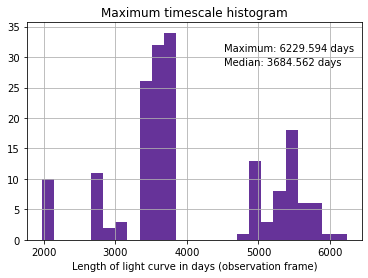
\includegraphics[width=0.46\linewidth]{Figures/MaxTimescale.png} }}%
    \qquad
    \subfloat{{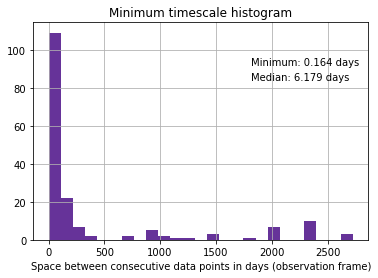
\includegraphics[width=0.46\linewidth]{Figures/MinTimescale.png} }}%
     \caption{Ιστογράμματα των μέγιστων και ελάχιστων χρονικών κλιμάκων. Αριστερά: ιστόγραμμα κατανομής των μηκών καμπύλων φωτός για όλες τις πηγές του πεδίου \textlatin{XMM-XXLL-N} που μελετάμε στο αδρανειακό σύστημα παρατήρησης, με τον διάμεσο αυτών να αποτελεί την μέγιστη χρονική κλίμακά μας. Δεξιά: ιστόγραμμα κατανομής των διαστημάτων μεταξύ διαδοχικών σημείων καμπύλων φωτός για όλες τις πηγές του πεδίου \textlatin{XMM-XXLL-N} που μελετάμε στο αδρανειακό σύστημα παρατήρησης, με τον διάμεσο αυτών να αποτελεί την ελάχιστη χρονική κλίμακά μας.} \label{fig:MaxMInTime}
\end{figure*}
 
Ως μέγιστη κλίμακα χρόνου $Τ_{max, mod}= 1/f_{min}$ για το μοντέλο μας επιλέγουμε το μέγιστο χρονικό διάστημα $\Delta T_{lightcurve}$ που εκτείνεται η καμπύλη φωτός μιας πηγής (απόσταση του πρώτου από το τελευταίο σημείο), όπως το καταγράφουμε στο αδρανειακό σύστημα παρατήρησης. Για τις πηγές του πεδίου που μελετάμε, η μέγιστη αυτή χρονική κλίμακα σε σύστημα ηρεμίας είναι $Τ_{max, mod}= 3684.562 \mbox{\textlatin{ days}}$ (όπως φαίνεται στο σχήμα \ref{fig:MaxMInTime}). Aυτός είναι ο διάμεσος του μήκους των καμπυλών φωτός στο σύστημα παρατήρησης του πληθυσμό που μελετάμε.\\
Ως ελάχιστη κλίμακα χρόνου $Τ_{min, mod}= 1/f_{max}$ για τα μοντέλα μας επιλέγουμε το ελάχιστο χρονικό διάστημα μεταξύ διαδοχικών σημείων μιας καμπύλης φωτός, για τις καμπύλες φωτός των πηγών του δείγματός μας όπως το καταγράφουμε στο αδρανειακό σύστημα παρατήρησης. Βρίσκουμε τον αριθμητικό διάμεσο των διαστημάτων μεταξύ διαδοχικών σημείων καπμύλων φωτός ο οποίος είναι $Τ_{min, mod}=6.179  \mbox{\textlatin{ days}}$ (όπως φαίνεται στο σχήμα \ref{fig:MaxMInTime}). 
Έτσι στην  εφαρμογή των μοντέλων που κάνουμε χρησιμοποιούμε ως μέγιστη χρονική κλίμακα $Τ_{max, mod}= 3684.562 \mbox{\textlatin{ days}}$ και ως ελάχιστη χρονική κλίμακα $Τ_{min, mod}= 6.179  \mbox{\textlatin{ days}}$. \\
Εισάγουμε τους χρόνους στο σύστημα παρατήρησης, αφού ο αλγόριθμος της εργασίας \cite{VAR} αναλαμβάνει διορθώσεις για το αδρανειακό σύστημα ηρεμίας των πηγών.

Όπως έχει επισημανθεί, σύμφωνα με μελέτες\cite{2013ApJ...771....9A}, η μεροληψία (\textlatin{bias}) στην εκτίμηση της \textlatin{ensemble NXSV} είναι σημαντική όταν η ελάχιστη συχνότητα ολοκλήρωσης (που συνδέεται με την μέγιστη χρονική κλίμακα $f_{min} =1/Τ_{max, mod}$) είναι μεγαλύτερη της συχνότητας αποκοπής $f_b$ των \textlatin{PSD} των μοντέλων. 
H ελάχιστη συχνότητα για την μελέτη μας είναι $$f_{min} =\frac{1}{Τ_{max, mod}} = \frac{1}{3684.562 \mbox{\textlatin{ days}} } = 3.1 \times 10^{-9}\; \mbox{\textlatin{s}}^{-1}$$ 
Για κάθε ένα μοντέλο κάνουμε το διάγραμμα πυκνότητας της συχνότητας αποκοπής $f_b$ με την λαμπρότητα $L_X$ στο ενεργειακό παράθυρο $0.2-2$ \textlatin{keV} χαράζοντας και το επίπεδο $f_{min} = 3.1 \times 10^{-9}$ \textlatin{s}$^{-1}$. Εξετάζουμε έτσι αν υπάρχει σημαντική μεροληψία στον υπολογισμό μας.
\begin{figure*}%
    \centering
    \subfloat{{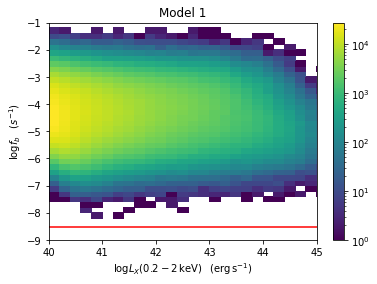
\includegraphics[width=0.46\linewidth]{Figures/Model 1 obs.png} }}%
    \qquad
    \subfloat{{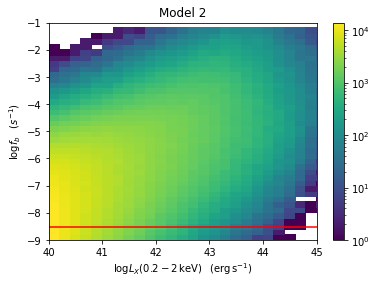
\includegraphics[width=0.46\linewidth]{Figures/Model 2 obs.png} }}%
    \vspace{4ex}
    \subfloat{{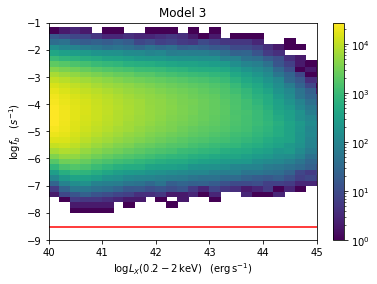
\includegraphics[width=0.46\linewidth]{Figures/Model 3 obs.png} }}
    \qquad
    \subfloat{{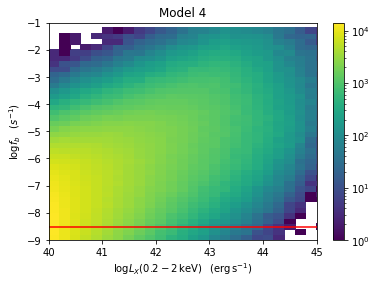
\includegraphics[width=0.46\linewidth]{Figures/Model 4 obs.png} }} \caption{Διαγράμματα πυκνότητας της συχνότητας αποκοπής $f_b$ (κατακόρυφος άξονας) με λαμπρότητα $L_X$ στο ενεργειακό παράθυρο $0.2-2$ \textlatin{keV} για κάθε ένα από τα τέσσερα Μοντέλα (σε κάθε πάνελ), η συχνότητα αποκοπής έχει μετασχηματιστεί για το αδρανειακό σύστημα παρατήρησης. Η κόκκινη γραμμή αντιπροσωπεύει την ελάχιστη συχνότητα ολοκλήρωσης της \textlatin{PSD:} $f_{min} = 3.1 \times 10^{-9}$ \textlatin{s}$^{-1}$ η οποία βασίζεται στην μέση μέγιστη χρονική κλίμακα στο σύστημα παρατήρησης. Οι άξονες του γραφήματος είναι σε λογαριθμική κλίμακα.} \label{fig:BiasModels}
\end{figure*}
 
'Οπως φαίνεται από το σχήμα \ref{fig:BiasModels}, gia τα Μοντέλα 1 και 3 δεν έχουμε σημαντικό \textlatin{bias} στον υπολογισμό της $\sigma_{rms}^2$, όμως για τα Μοντέλα 2 και 3 στις λαμπρότητες $10^{40}-10^{45}$ \textlatin{erg  s}$^{-1}$ βλέπουμε ότι έχουμε συχνότητες αποκοπής μικρότερες της ελάχιστης συχνότητας ολοκλήρωσης, οπότε έχουμε σημαντικό \textlatin{bias} στον υπολογισμό της $\sigma_{rms}^2$ από φαινόμενα \textlatin{aliasing} από χαμηλότερες συχνότητες. Ο αλγόριθμος που υπολογίζει την \textlatin{ensemble NXSV} me ολοκλήρωση των \textlatin{PSD} διορθώνει την $\sigma_{rms}^2$ με πολλαπλασιαστικό παράγοντα $C \cdot 0.48^{\beta-1}$, λαμβάνοντας τιμές $C = 1.3$ kai $\beta = 1.1$. 

Καταλήγουμε στην παραγωγή τεχνητού δείγματος \textlatin{AGN} με \textlatin{redshift} $z \in [0,4]$ kai λαμπρότητα $L_X$ στο ενεργειακό παράθυρο $[0.2 \mbox{\textlatin{keV}}\;, 2 \; \mbox{\textlatin{keV}}]$ για κάθε μοντέλο \textlatin{PSD}, για το οποίο υπολογίζουμε πλάτος μεταβλητότητας $\sigma_{rms, mod}^2$  ολοκληρώνοντας τις \textlatin{PSD} των μοντέλων για παρατηρούμενες χρονικές κλίμακες $Τ_{min, mod}= 6.179 \mbox{\textlatin{ days}}$ kai $Τ_{max, mod} = 3684.562  \mbox{\textlatin{ days}}$. Συνυπολογίζεται διόρθωση \textlatin{bias}. 
 
\begin{figure*}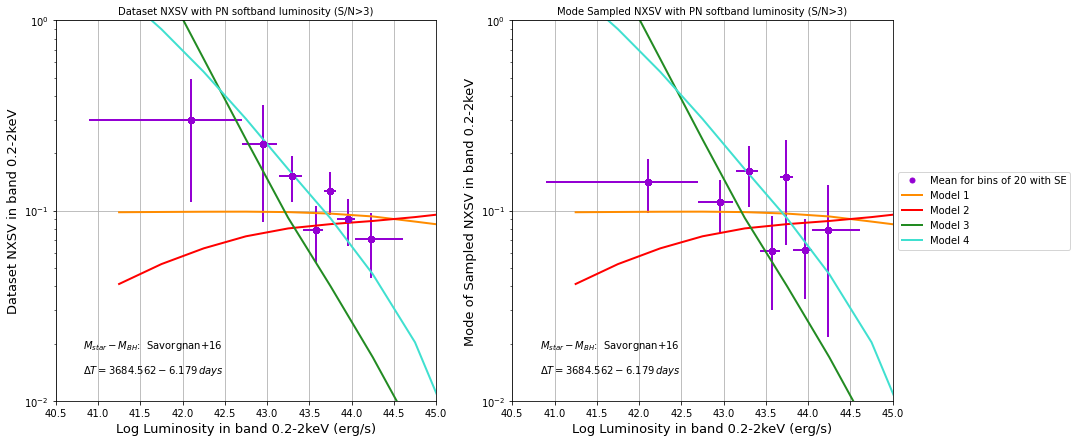
\includegraphics[width=1.1\linewidth]{Figures/ModelsFINAL.png}\caption{Αριστερά: η \textlatin{NXSV} όπως υπολογίσαμε από τα δεδομένα αρχείου με λαμπρότητα και \textlatin{binning} κατά λαμπρότητα σε \textlatin{bin} των 20 πηγών με διαφοροποίηση για \textlatin{redshift} και τα Μοντέλα 1, 2, 3, 4 διαφοροποιούνται στην μορφή της \textlatin{PSD} όπως έχει επισημανθεί, η ελάχιστη χρονική κλίμακα μεταβλητότητας είναι $Τ_{min, mod}=  6.179 \mbox{\textlatin{ days}}$, δηλαδή ο διάμεσος των μικρότερων χρονικών αποστάσεων ηρεμίας διαδοχικών σημείων καμπύλης φωτός μεταξύ των πηγών και η μέγιστη χρονική κλίμακα είναι η μέγιστη όλων των καμπύλων φωτός $Τ_{max, mod}=  3684.562 \mbox{\textlatin{ days}}$. Δεξιά: η \textlatin{NXSV} από τον αλγόριθμο \textlatin{Bayes} όπως έχει περιγραφεί με λαμπρότητα και τα ίδια ακριβώς φασματικά μοντέλα. }  \label{fig:ModelsFinal} \end{figure*}

\begin{figure*}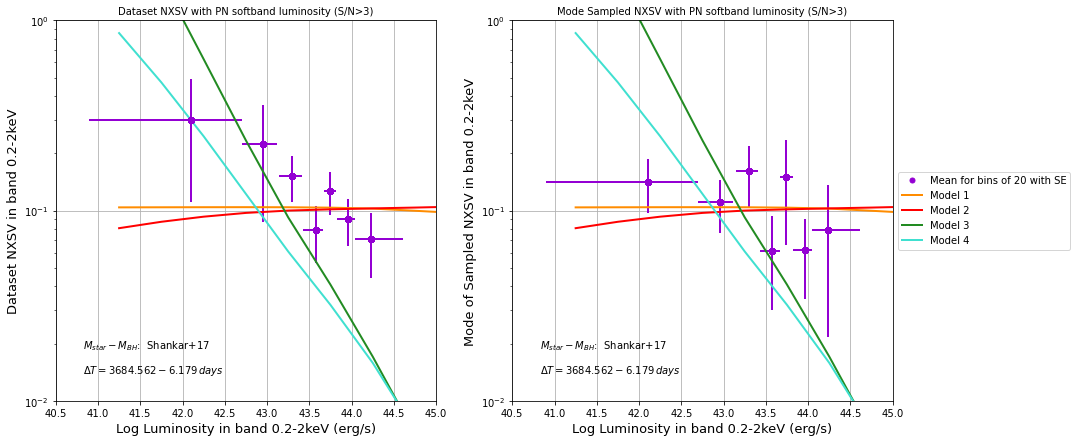
\includegraphics[width=1.1\linewidth]{Figures/ModelsFINALshankar.png}\caption{Αριστερά: η \textlatin{NXSV} όπως υπολογίσαμε από τα δεδομένα αρχείου με λαμπρότητα και \textlatin{binning} κατά λαμπρότητα σε \textlatin{bin} των 20 πηγών με διαφοροποίηση για \textlatin{redshift} και τα Μοντέλα 1, 2, 3, 4 διαφοροποιούνται στην μορφή της \textlatin{PSD} όπως έχει επισημανθεί, εδώ αυτή τη φορά αντί να χρησιμοποιήσουμε την σχέση αστρικής μάζας με μάζα μελανής οπής όπως προτείνεται από την εργασία \cite{savorgnan}, χρησιμοποιούμε την συσχέτιση μαζών σύμφωνα με την εργασία \cite{shankar}. Δεξιά: η \textlatin{NXSV} από τον αλγόριθμο \textlatin{Bayes} όπως έχει περιγραφεί με φωτεινότητα και τα ίδια ακριβώς φασματικά μοντέλα. }  \label{fig:ModelsFinalshankar} \end{figure*}

Στο σχήμα \ref{fig:ModelsFinal} χαράσουμε την σχέση πλάτους μεταβλητότητας με λαμπρότητα στις μαλακές ακτίνες Χ για κάθε μοντέλο (συνεχής γραμμή με χρωματικό κώδικα για Μοντέλο 1, Μοντέλο 2, Μοντέλο 3, Μοντέλο 4) για το τεχνητό δείγμα \textlatin{AGN} με τα χαρακτηριστικά που συζητήσαμε, και τοποθετούμε την \textlatin{ensemble NXSV} για ομάδες 20 τουλάχιστον πηγών του πληθυσμό \textlatin{AGN} του πεδίου \textlatin{XMM-XXL-North} όπως την υπολογίσαμε από δεδομένα αρχείου (επιλέγοντας πηγές με λόγο \textlatin{S/N}$>3$ και με διαθέσιμη τιμή \textlatin{redshift}) kai την \textlatin{ensemble NXSV} για ομάδες 20 τουλάχιστον \textlatin{AGN} από τον δειγματολογικό αλγόριθμο \textlatin{Bayes} που βασίσαμε στις πηγές του πληθυσμού \textlatin{AGN} του πεδίου \textlatin{XMM-XXL-North}. Στο σχήμα \ref{fig:ModelsFinal} η συνάρτηση αστρικής μάζας κεντρικού σφαιροειδούς με την μάζα υπερμεγέθους μελανής οπής που χρησιμοποιήθηκε στον τεχνητό πληθυσμό μας είναι η (\textlatin{Savorgnan})\cite{savorgnan} 
$$ \log_{10} \frac{M_{BH}}{M_\odot} = 8.35 +1.31 (\log_{10} \frac{M_\star}{M_\odot} +11.0) $$
ενώ, για σύγκριση, χαράσουμε το ίδιο διάγραμμα στο σχήμα \ref{fig:ModelsFinalshankar} ακολουθώντας για τον πληθυσμό μας την εναλλακτική σχέση (\textlatin{Shankar})\cite{shankar} 
$$ \log \frac{M_{BH}}{M_\odot} = 7.574 +  1.946(\log \frac{M_\star}{M_\odot} +11.0)  -0.306(\log \frac{M_\star}{M_\odot} +11.0)^2 -0.011(\log \frac{M_\star}{M_\odot} +11.0) ^3 $$

%(Στην εργασία αυτή, όταν χρησιμοποιούμε το σύμβολο του λογαρίθμου εννοούμε δεκαδικό λογάριθμο- εκτός αν τονίζεται διαφορετικά.)\\
Παρατηρούμε ότι στην περίπτωση του κλασσικού υπολογισμού της \textlatin{ensemble NXSV} από την βάση δεδομένων το Μοντέλο 1 περνά από τις γραμμές σφαλμάτων 5 σημείων απο τα 7, ενώ το Μοντέλο 4 περνά από τις γραμμές σφάλματος 4 σημείων από τα 7. Στον υπολογισμό της \textlatin{ensemble NXSV} από τον δειγματοληπτικό αλγόριθμο συμπερασματολογίας \textlatin{Bayes} τόσο το Μοντέλο 1 όσο και και το Μοντέλο 4 περνούν από τις γραμμές σφάλματος 4 σημείων από τα 7 (αναφερόμαστε πρωτίστως στα μοντέλα με χρήση της σχέσης μάζας \textlatin{Savorgnan} που θεωρείται πιο έγκυρη- χρησημοποιούμε την σχέση μάζας \textlatin{Shankar} αμιγώς για σύγκριση).

Λόγω των μεγάλων σφαλμάτων των μετρήσεων είναι δύσκολο να βγάλουμε συμπεράσματα για το ποιό μοντέλο περιγράφει καλύτερα τα δεδομένα μας.\\
Εφαρμόζουμε το στατιστικό τεστ $\chi^2$ καλύτερης προσαρμογής, το οποίο λαμβάνει υπ> όψιν την αβεβαιότητα στις μετρήσεις ως εξής
$$ \chi^2 = \sum_{i=1}^N \Big( \dfrac{x_{obs} - x_{model}}{\sigma_i} \Big)^2$$
με $x_{obs}$ τις μετρήσεις της \textlatin{ensemble NXSV}, $x_{model}$ την τιμή της \textlatin{NXSV} που προτείνει το εκάστοτε μοντέλο για την ίδια λαμπρότητα και $\sigma_i$ η κανονική απόκλιση (\textlatin{standard deviation})- η οποία σχετίζεται αλλά δεν είναι το ίδιο το κανονικό σφάλμα (\textlatin{standard error}) των μετρήσεων μας. Το μοντέλο που προσαρμόζεται καλύτερα στα δεδομένα μας είναι αυτό με την μικρότερη ποσότητα $\chi^2$. Έπειτα εφαρμόζουμε το τεστ $\chi^2$ ανά βαθμό ελευθερίας (\textlatin{Reduced} $\chi^2$), όπου υπολογίζουμε την ποσότητα $$\chi_\nu^2= \frac{\chi^2}{\nu}$$ gia $\nu$ βαθμούς ελευθερίας. Το τεστ αυτό εγγυάται ότι δεν οδηγηθήκαμε σε λάθος αποτέλεσμα λόγω μερικών παθολογικών σημείων στα δεομένα μας.\\
Εφαρμόζοντας το τεστ $\chi^2$ και το \textlatin{reduced} $\chi^2$ προκύπτουν οι πίνακες\\

\begin{tabular}{ |p{3cm}||p{4.5cm}|p{4.5cm}|  }
 \hline
 \multicolumn{3}{|c|}{$\chi^2$ για την κλασσική \textlatin{ensemble NXSV}} \\
 \hline
 Μοντέλο & με σχέση μάζας \textlatin{Savorgnan} & με σχέση μάζας \textlatin{Shankar}\\
 \hline
 Μοντέλο 1 & 0.239148 & 0.238390\\
 Μοντέλο 2 & 0.353530 & 0.274656\\
 Μοντέλο 3 &  1.504368 & 1.495005\\
 Μοντέλο 4 & 0.859485 & 1.592550\\
 \hline
\end{tabular}\\

\begin{tabular}{ |p{3cm}||p{4.5cm}|p{4.5cm}|  }
 \hline
 \multicolumn{3}{|c|}{$\chi^2$ για την \textlatin{bayesian ensemble NXSV}} \\
 \hline
 Μοντέλο & με σχέση μάζας \textlatin{Savorgnan} & με σχέση μάζας \textlatin{Shankar}\\
 \hline
 Μοντέλο 1 &  0.211197 & 0.251096\\
 Μοντέλο 2 & 0.369378 & 0.293122\\
 Μοντέλο 3 &  5.696387 & 5.616701\\
 Μοντέλο 4 & 4.780370 & 0.727012\\
 \hline
\end{tabular}\\    \\

 

\begin{tabular}{ |p{3cm}||p{4.5cm}|p{4.5cm}|  }
 \hline
 \multicolumn{3}{|c|}{$\chi_\nu^2$ για την κλασσική \textlatin{ensemble NXSV}} \\
 \hline
 Μοντέλο & με σχέση μάζας \textlatin{Savorgnan} & με σχέση μάζας \textlatin{Shankar}\\
 \hline
 Μοντέλο 1 &  0.034164 & 0.034056\\
 Μοντέλο 2 & 0.050504 & 0.039237\\
 Μοντέλο 3 &  0.214909 & 0.213572\\
 Μοντέλο 4 & 0.122784 & 0.227507\\
 \hline
\end{tabular}\\

\begin{tabular}{ |p{3cm}||p{4.5cm}|p{4.5cm}|  }
 \hline
 \multicolumn{3}{|c|}{$\chi_\nu^2$ για την \textlatin{bayesian ensemble NXSV}} \\
 \hline
 Μοντέλο & με σχέση μάζας \textlatin{Savorgnan} & με σχέση μάζας \textlatin{Shankar}\\
 \hline
 Μοντέλο 1 &  0.030171 & 0.035870\\
 Μοντέλο 2 & 0.052768 & 0.041875\\
 Μοντέλο 3 &  0.813769 & 0.802386\\
 Μοντέλο 4 & 0.682910 & 0.103859\\
 \hline
\end{tabular}\\ \\

Βλέπουμε ότι το Μοντέλο 1 είναι αυτό με την καλύτερη προσαρμογή τοσο για την κλασσική \textlatin{ensemble NXSV} όσο και για την \textlatin{bayesian ensemble NXSV}, έχει συστηματικά την μικρότερη ποσότητα $\chi^2$ και $\chi_\nu^2$ για οποιαδήποτε συνάρτηση μάζας.\\
Τα υπόλοιπα μοντέλα φαίνεται να υπολείπονται των παρατηρήσεων, όμως ασφαλέστερα συμπεράσματα για καθαρή προσαρμογή με τα δεδομένα μας θα μπορούσαμε να βγάλουμε αν είχαμε μικρότερα σφάλματα- δηλαδή επιπλέον παρατηρήσεις (αφού στις μετρήσεις της \textlatin{ensemble NXSV} τα σφάλματα είναι στατιστικά).

%({\color{red} Θα ελεγα οτι το λογω των μεγαλαων σφαλματων των μετρησεων ειναι δυσκολο να βγαλεις συμπερασμα, αλλα φαινεται οτι το μοντελο που φαινεται να περιγραφεις τις παρατηρησεις ειναι το Μοντελο -1 ανεξαρητηα κλασσικης ή Μπαυζοαμης. Τα υπολοιπα μοντελα φαινονται να υπολειπονται των ποαρατηρησεψν, αλλα μικροτερα σφαλματα (επιπλεον παρατηρησεις) ειναι απααιτηρητες για ασφαλη συμεπρασματα.})..